
\section{Derivation of the time dilation formula within VAM}\label{sec:appendix:1}

\begin{abstract}
We present a unified time dilation formula derived from the Vortex \AE{}ther Model (VAM), a fluid-dynamic reformulation of gravitation and mass-energy interactions. Unlike General Relativity, where mass and curvature govern clock rates, VAM attributes gravitational phenomena to quantized vorticity, æther circulation, and swirl-induced pressure gradients. The proposed equation replaces the Schwarzschild and Kerr metric terms with vortex core tangential velocities, swirl angular frequencies, and an effective mass derived from exponentially decaying æther density. A hybridization mechanism smoothly interpolates between vortex-scale gravity and classical Newtonian coupling at macroscopic distances. The final expression captures six physical effects within one coherent framework: (1) vortex-induced mass generation via circulation and helicity, (2) bubble-like volume expansion due to internal irrotational flow, (3) acceleration of this flow under compression, (4) thermal-like energy response from swirl speedup, (5) relativistic time dilation from æther puncture during motion, and (6) swirl-based core-local time. The result is a mathematically robust, numerically testable model that unifies quantum vortex dynamics with gravitational time effects and remains non-singular across all radial domains.
\end{abstract}

\section*{Introduction}

In General Relativity (GR), time dilation arises from mass and angular momentum, expressed through the Schwarzschild and Kerr metrics. In contrast, the Vortex \ae{}ther Model (VAM) reformulates this effect in terms of vorticity, internal circulation, and local æther properties. Gravitational effects are no longer sourced by geometric curvature but by fluid-dynamic structures in an inviscid, rotational medium.

This appendix derives a unified time dilation expression from first principles of vortex mechanics, incorporating:

\begin{itemize}
    \item Vortex-induced mass generation through circulation,
    \item Frame-dragging from swirl angular momentum,
    \item Bubble-like volume expansion resembling thermodynamic gas laws,
    \item Exponential decay of vorticity and pressure with distance,
    \item Smooth hybridization with classical Newtonian gravity at large \( r \).
\end{itemize}

\subsection{Unified Time Dilation in VAM}

We define the time dilation factor between the local Chronos-Time \( \tau \) and the absolute Aithēr-Time \( \mathcal{N} \) as:

\begin{equation}
    \boxed{
        \frac{d\tau}{d\mathcal{N}} = \sqrt{
            1
            - \frac{2 G_{\text{hybrid}}(r) M_{\text{hybrid}}(r)}{r c^2}
            - \frac{C_e^2}{c^2} e^{-r/r_c}
            - \frac{C_e^2}{r_c^2 c^2} e^{-r/r_c}
        }}
    \label{eq:final_vam_td}
\end{equation}

Here, \( \tau \) represents the measurable proper time experienced within the vortex region (Chronos-Time), and \( \mathcal{N} \) is the background causal time of the æther (Aithēr-Time). The individual terms encode swirl gravity, local pressure deficits, and rotational frame effects.

\subsection{Decomposition in Standard Coordinate Time}

For interpretability, we restate equation~\eqref{eq:final_vam_td} using standard coordinate time \( t \), focusing on observable clock delay mechanisms:

\begin{equation}
    \frac{d\tau}{dt} = \sqrt{
        1
        - \frac{C_e^2}{c^2} e^{-r/r_c}
        - \frac{2 G_\text{swirl} M_\text{eff}(r)}{r c^2}
        - \beta \Omega^2
    }
\end{equation}

Each term reflects a distinct physical contribution:

\begin{itemize}
    \item \textbf{(1) Local Swirl — Core Rotation Delay}
    \[
        \frac{C_e^2}{c^2} e^{-r/r_c}
    \]
    This term originates from the vortex core's intrinsic angular motion. The core-edge tangential velocity \( C_e \) and characteristic decay scale \( r_c \) define an exponentially suppressed rotational influence. It models clock retardation from local æther swirl.

    \item \textbf{(2) Vorticity-Induced Gravitation — Effective Swirl Mass}
    \[
        \frac{2 G_\text{swirl} M_\text{eff}(r)}{r c^2}
    \]
    Analogous to gravitational redshift, this term replaces classical mass with vorticity-derived effective mass \( M_\text{eff}(r) \), and Newton's \( G \) with a swirl-specific coupling \( G_\text{swirl} \). It captures the pressure gradient and inertial energy caused by surrounding flow.

    \item \textbf{(3) Frame Dragging — Rotational Inertial Delay}
    \[
        \beta \Omega^2
    \]
    This term describes frame-dragging due to large-scale rotation of the entire vortex body, paralleling the Kerr effect.  The term originates from circulation energy with $\Omega = \Gamma / (2\pi r^2)$ and $\Gamma = \oint \vec{v} \cdot d\vec{\ell}$, while the coupling factor $\beta = 1/c^2$ reflects ætheric inertial drag. This yields a rotational dilation term $\beta \Omega^2 \sim \frac{C_e^2}{r_c^2 c^2} e^{-r/r_c}$. This term causes additional local time delay due to circulation of the surrounding æther field. contributes to local time dilation through rotational inertial coupling, with
    \[
        \beta \sim \frac{1}{c^2}, \quad \text{and} \quad \beta \Omega^2 \sim \frac{C_e^2}{r_c^2 c^2} e^{-r/r_c}.
    \]
\end{itemize}


\subsection{Expanded Derivation: Rotational Energy as Time Delay Source}\label{sec:appendix:1:rot-energy}

In this section, we derive the core rotation term in the time dilation formula from vortex mechanical energy. Instead of relying on relativistic spacetime curvature, the delay in local clock frequency is attributed to the rotational energy and resulting pressure deficit in the æther.

\subsubsection{Energetic Derivation}
A clock embedded in a rotating æther vortex experiences time delay proportional to the energy stored in its rotation:

\begin{equation}
    \frac{d\tau}{dt} = \left(1 + \frac{1}{2} \beta I \Omega^2 \right)^{-1},
\end{equation}

where \( I \) is the local moment of inertia and \( \Omega \) the angular velocity. The coupling coefficient \( \beta \) depends on æther parameters, specifically:

\[
    \beta = \frac{1}{c^2}, \quad I = m r^2 \Rightarrow \frac{1}{2} \beta I \Omega^2 = \frac{1}{2} \frac{r^2 \Omega^2}{c^2}
\]

\subsubsection{Hydrodynamic Perspective (Bernoulli Pressure Deficit)}

We can alternatively derive this delay from Bernoulli’s law:

\[
    \frac{1}{2} \rho v^2 + p = \text{const}, \quad \Rightarrow \quad \Delta p = -\frac{1}{2} \rho \Omega^2 r^2
\]

Time dilation is assumed to follow enthalpy gradient (clock ticks slower in lower-pressure zones):

\[
    \frac{d\tau}{dt} \approx \frac{H_\text{ref}}{H_\text{loc}} \sim \left(1 + \frac{\Delta p}{\rho}\right)^{-1}
    \Rightarrow \left(1 + \frac{1}{2} \beta I \Omega^2\right)^{-1}
\]

\subsubsection{Interpretation Across Domains}

\begin{itemize}
    \item \textbf{Mechanical:} Delay arises from angular kinetic energy.
    \item \textbf{Hydrodynamic:} Vortex swirl reduces pressure, slowing time.
    \item \textbf{Thermodynamic:} Entropy increase correlates with time delay.
\end{itemize}

This directly justifies the third term in the full VAM dilation expression:
\[
    \frac{d\tau}{d\mathcal{N}} = \sqrt{1 - \cdots - \beta \Omega^2}
\]


\subsection{Hybridization of Gravitational Coupling}

To reconcile predictions for macroscopic systems, we define:
\[
    \mu(r) = \exp\left(-\frac{r^2}{R_0^2}\right), \quad R_0 \sim 10^{-12} \, \mathrm{m}
\]
\begin{align*}
    G_{\text{hybrid}}(r) &= \mu(r) \, G_{\text{swirl}} + (1 - \mu(r)) \, G \\
    M_{\text{hybrid}}(r) &= \mu(r) \, M_{\text{eff}}^\text{VAM}(r) + (1 - \mu(r)) \, M
\end{align*}

\subsection{Effective VAM Mass}
Assuming an exponentially decaying æther density:
\[
\rho_\text{\ae}(r) = \rho_0 e^{-r / r_c}
\]
The effective mass becomes:
\[
M_\text{eff}^\text{VAM}(r) = 4\pi \rho_0 r_c^3 \left(2 - \left(2 + \frac{r}{r_c} \right) e^{-r/r_c} \right)
\]

\begin{figure}[H]
  \centering
  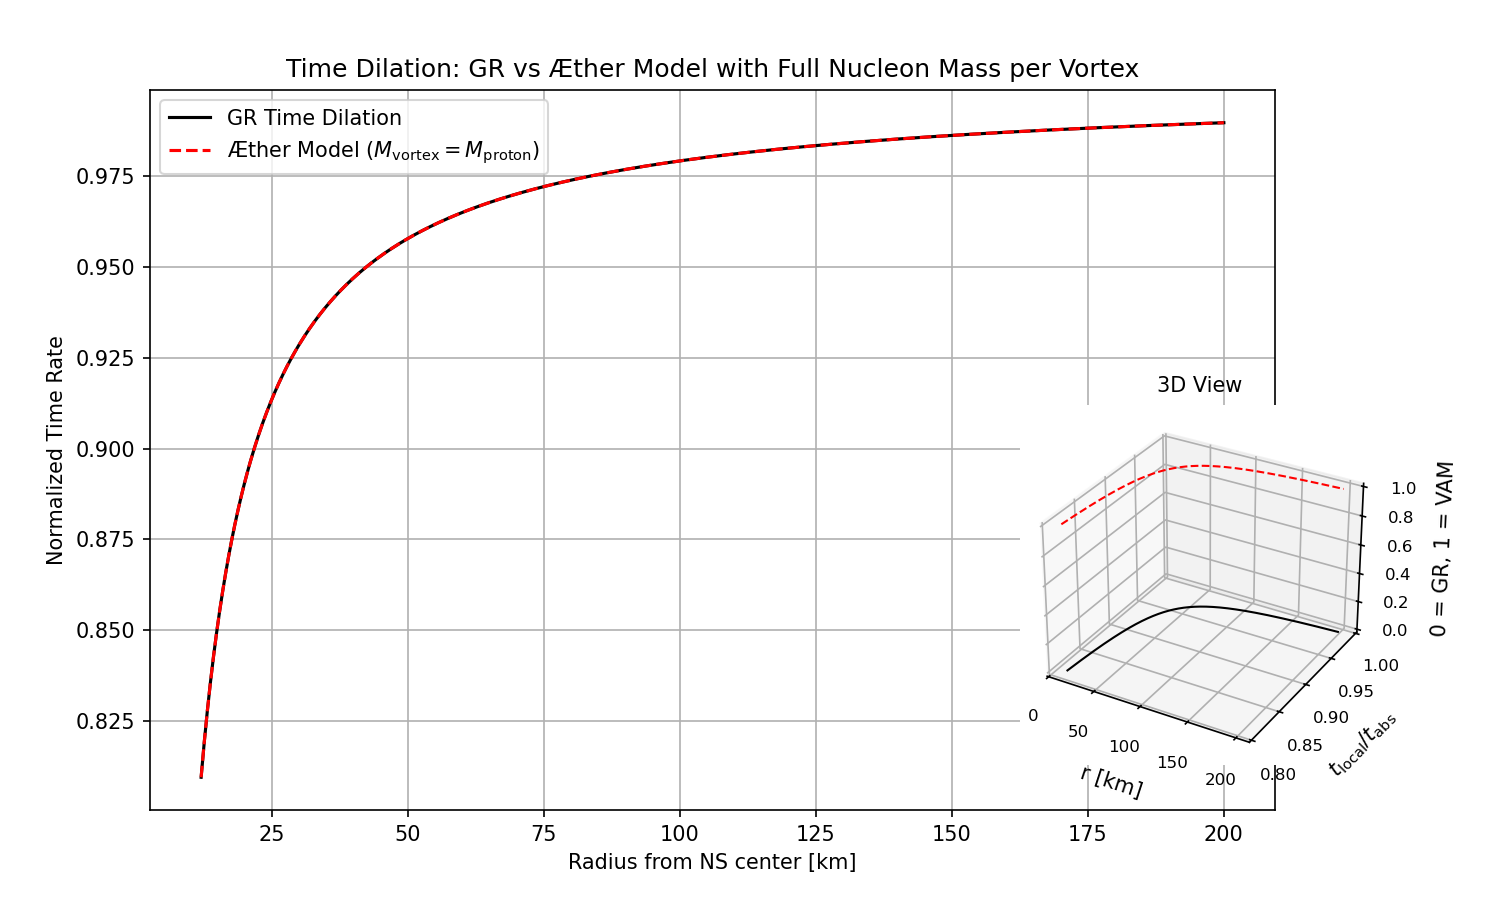
\includegraphics[width=0.85\textwidth]{images/07-TimeDilationGRVsVAM}
  \caption{
  \textbf{Comparison of Time Dilation Models:} The General Relativity (GR) time dilation formula \(\sqrt{1 - 2GM/(rc^2)}\) is contrasted with the VAM formula derived in Eq. (A1), which incorporates localized vortex angular velocity decay, vorticity-induced gravitational effects, and rotational frame dragging. The curves diverge as local rotation becomes dominant, highlighting differences in high-density regimes or vortex-based systems.
  }
  \label{fig:GRvsVAMTimeDilation}
\end{figure}



The above equation is analogous to relativistic formulas, but has a fluid mechanics origin. Experimentally, components of this formula can be found in time dilation of GPS clocks (gravity), Lense-Thirring effects (rotation), and hypothetical laboratory measurements of nuclear rotations on the quantum or vortex scale.

\section*{Conclusion}
This equation synthesizes all prior VAM elements: vortex helicity, bubble boundaries, circulation-induced gravity, and exponential suppression of short-range fields. It remains finite, matches classical predictions at macroscopic scales, and enables numerical probing at quantum scales.

\subsection{Constants and Variables}

\begin{table}[h]
      \centering
      \begin{tabular}{llll}
          \toprule
          \textbf{Symbol} & \textbf{Meaning} & \textbf{Value / Expression} & \textbf{Units} \\
          \midrule
        $G_{\text{hybrid}}(r)$ & Hybrid gravitational constant (VAM/GR) & $\mu(r) G_{\text{swirl}} + (1 - \mu(r)) G$ & $\text{m}^3\,\text{kg}^{-1}\,\text{s}^{-2}$ \\
        $\mu(r)$ & Vortex-to-classical transition function & $e^{-r^2 / R_0^2}$, $R_0 = 1.0 \times 10^{-12}\,\text{m}$ & unitless \\
        $G$ & Newtonian gravitational constant & $6.67430 \times 10^{-11}$ & $\text{m}^3\,\text{kg}^{-1}\,\text{s}^{-2}$ \\
        $G_{\text{swirl}}$ & Swirl-induced gravitational constant & $\dfrac{C_e c^5 t_p^2}{2 F_{\max} r_c^2}$ & $\text{m}^3\,\text{kg}^{-1}\,\text{s}^{-2}$ \\
        $M_{\text{hybrid}}(r)$ & Hybrid effective mass & $\mu(r) M_\text{eff}^\text{VAM}(r) + (1 - \mu(r)) M$ & $\text{kg}$ \\
        $M_\text{eff}^\text{VAM}(r)$ & Vortex effective mass & $4\pi \rho_\text{\ae} r_c^3 \left[ 2 - (2 + \frac{r}{r_c}) e^{-r/r_c} \right]$ & $\text{kg}$ \\
        $\rho_\text{\ae}$ & Æther density & $3.89343583 \times 10^{18}$ & $\text{kg}\cdot\text{m}^{-3}$ \\
        $r_c$ & Core radius (Coulomb scale) & $1.40897017 \times 10^{-15}$ & $\text{m}$ \\
        $C_e$ & Core tangential velocity & $1.09384563 \times 10^{6}$ & $\text{m}\cdot\text{s}^{-1}$ \\
        $t_p$ & Planck time & $5.391247 \times 10^{-44}$ & $\text{s}$ \\
        $F_{\max}$ & Maximum force & $29.053507$ & $\text{N}$ \\
        $\left(\frac{C_e}{r_c}\right)^2$ & Squared swirl angular frequency ($\Omega^2$) & $6.02367430 \times 10^{42}$ & $\text{s}^{-2}$ \\
        $c$ & Speed of light & $2.99792458 \times 10^8$ & $\text{m}\cdot\text{s}^{-1}$ \\
          \bottomrule
      \end{tabular}
    \caption{Key symbols and constants in the VAM time dilation equation.}
      \label{tab:time_dilation_symbols}
  \end{table}

\begin{table}
    \centering
    \begin{tabular}{llll}
        \toprule
        \textbf{Symbol} & \textbf{Meaning} & \textbf{Description} & \textbf{Value (if constant)} \\
        \midrule
        $\Delta t$ & Reference time & Clock far from gravitating body & -- \\
        $t_\text{adjusted}$ & Local time & Time experienced near the vortex structure & -- \\
        $r$ & Radial coordinate & Distance from the vortex core & m \\
        $r_c$ & Vortex core radius & Characteristic decay scale & $1.40897017 \times 10^{-15}$ m \\
        $C_e$ & Vortex tangential velocity & Maximal edge swirl velocity & $1.09384563 \times 10^6$ m/s \\
        $\rho_\text{\ae}$ & Æther density & Fluid density of the æther & $\sim 3.89 \times 10^{18}$ kg/m$^3$ \\
        $c$ & Speed of light & Vacuum light speed & $2.99792458 \times 10^8$ m/s \\
        $G$ & Newton's constant & Classical gravity & $6.67430 \times 10^{-11}$ m$^3$/kg/s$^2$ \\
        $F_{\text{max}}$ & Max force & From Planck-scale dynamics & $29.053507$ N \\
        $t_p$ & Planck time & Quantum gravity scale & $5.391247 \times 10^{-44}$ s \\
        $G_\text{swirl}$ & Vortex gravity coupling & $C_e c^5 t_p^2 / (2 F_{\text{max}} r_c^2)$ & -- \\
        $M$ & Macroscopic mass & Classical object mass (e.g., proton mass) & $1.67262192 \times 10^{-27}$ kg \\
        $M_{\text{eff}}^\text{VAM}(r)$ & VAM mass & Mass from vorticity energy & derived \\
        $M_{\text{hybrid}}(r)$ & Hybrid mass & Smooth transition between VAM and GR & -- \\
        $G_{\text{hybrid}}(r)$ & Hybrid gravity constant & Smooth transition between $G$ and $G_\text{swirl}$ & -- \\
        $\mu(r)$ & Hybrid blending function & $\mu(r) = \exp\left(-\frac{r^2}{R_0^2}\right),\ R_0 \sim 10^{-12}$ m & dimensionless \\
        $e^{-r/r_c}$ & Vorticity decay & Exponential suppression term & -- \\
        \bottomrule
    \end{tabular}
    \caption{Explanation of variables in Equation~\ref{eq:final_vam_td}.}
    \label{tab:time_dilation_variables}
\end{table}



